\documentclass[]{article}
\usepackage[pdftex,paperwidth=434pt,paperheight=262pt,noheadfoot,left=0pt,top=0pt]{geometry}
\usepackage{graphicx}

\begin{document}
\noindent
%\scalebox{0.8819}[0.8966]{
\begin{picture}(432,261)
\put(-108,-464){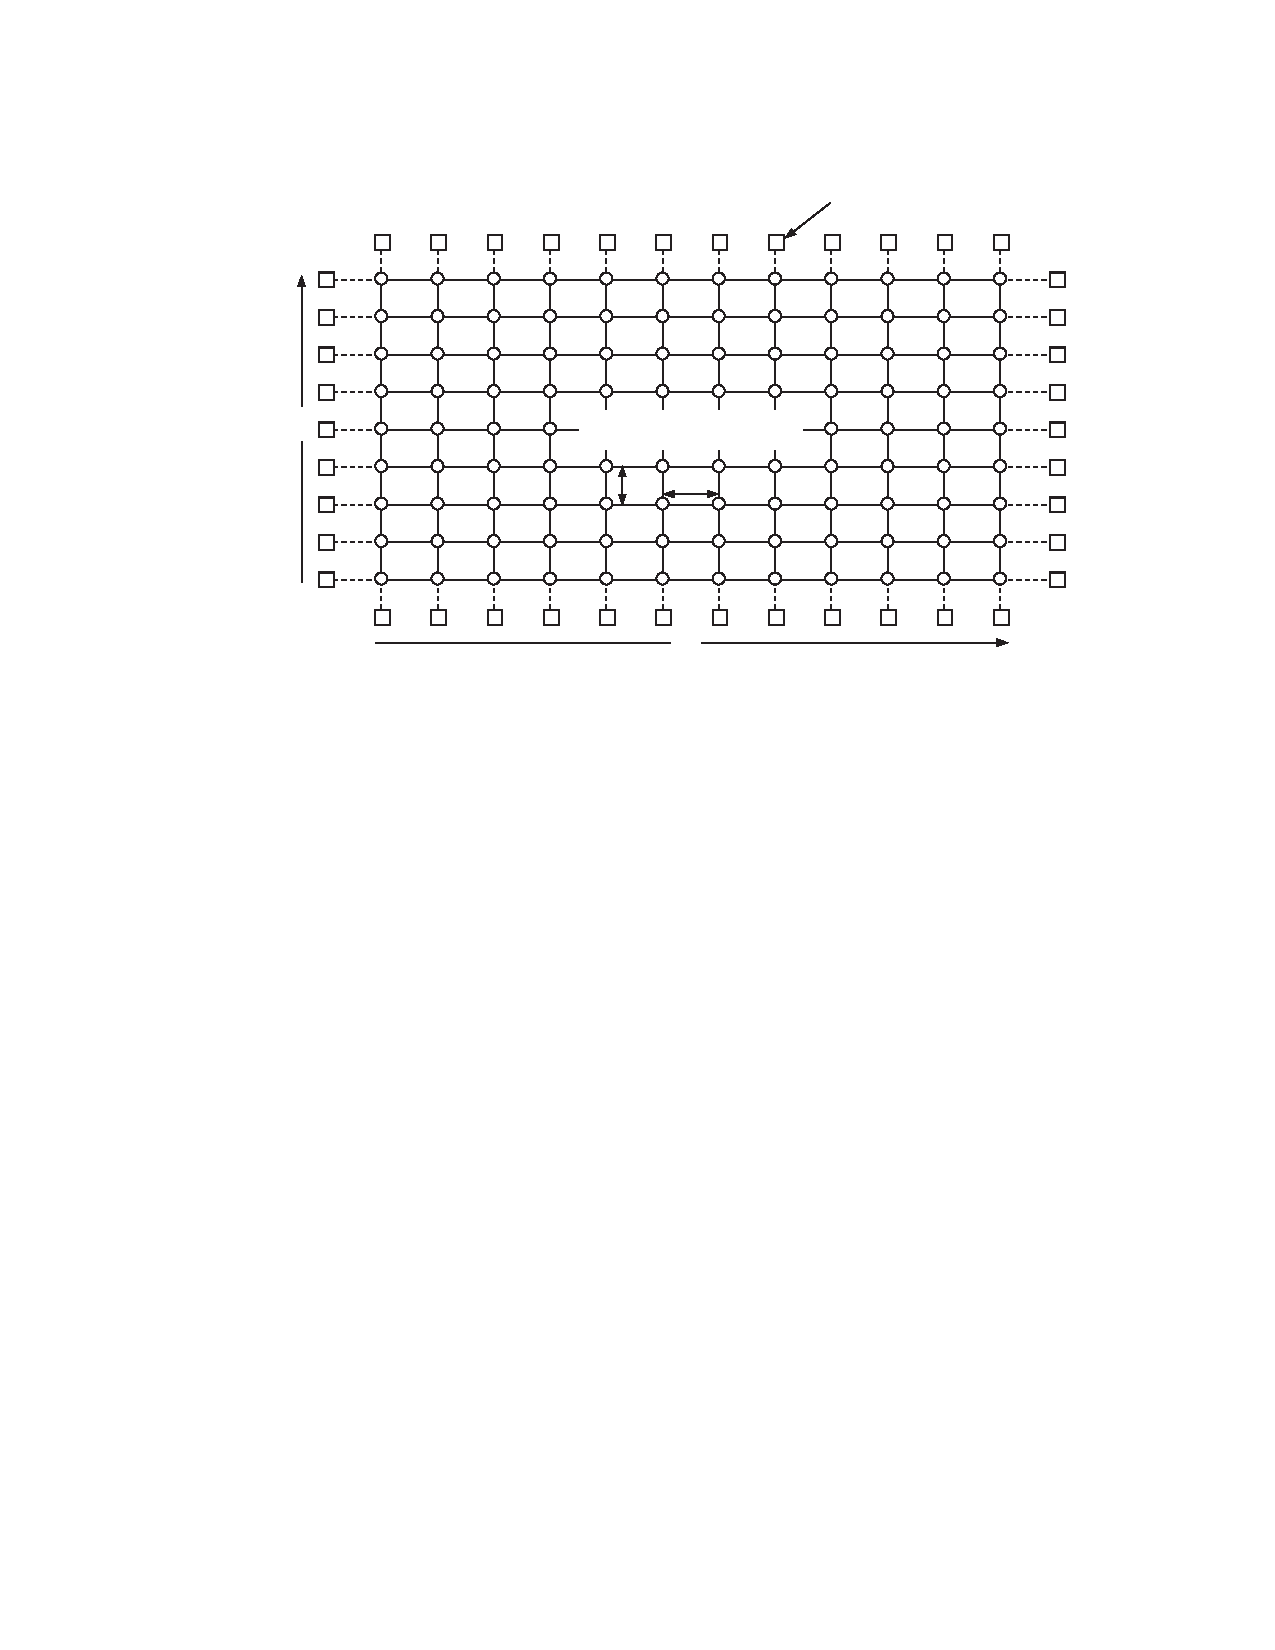
\includegraphics[width=8.5in]{PDFnotext/Figure8_1.pdf}}
\put(35,41){0}
\put(35,122){$\theta$}
\put(30,201){$\pi/2$}
\put(66,18){0}
\put(220,18){$x$}
\put(378,18){$x_f$}
\put(77,56){\scriptsize(0,0)}
\put(354,56){\scriptsize(${\cal I}$,0)}
\put(77,188){\scriptsize(0,${\cal J}$)}
\put(353,188){\scriptsize(${\cal I}$,${\cal J}$)}
\put(196,94){$h_\theta$}
\put(220,96){$h_x$}
\put(180,121){Computational Mesh}
\put(254,234){virtual boundary point}
\end{picture}
%}
\end{document}
